\documentclass[polish,12pt,a4paper]{extarticle}
\usepackage[T1]{fontenc}

\usepackage[top=2.5cm,bottom=2cm,left=2cm,right=2cm]{geometry}
\usepackage{xcolor}

\usepackage{placeins}  % in the preamble
\usepackage{babel}
\usepackage{titling}
\usepackage{lastpage}
\usepackage{amsmath}
\usepackage{amssymb}
\usepackage{stmaryrd}
\usepackage{fancyhdr}
\usepackage[bookmarks=false]{hyperref}
\usepackage{algorithm2e}
\usepackage{mathtools}
\usepackage{xcolor}
%\usepackage{overarrows}
\pagestyle{fancy}

\usepackage{tikz}
\usetikzlibrary{angles,quotes}

\title{Miniprojekt 1}
\author{Jakub Wieliczko}

\fancyhead[l]{MPUM}
\fancyhead[c]{\textbf{\thetitle}}
\fancyhead[r]{\theauthor}
\fancyfoot[c]{\begin{NoHyper}\thepage/\pageref{LastPage}\end{NoHyper}}

\newcommand{\inident}{\hspace{1.25em}}

% Algo stuff
\newcommand\mycommfont[1]{\ttfamily\textcolor{gray}{#1}}
\SetCommentSty{mycommfont}
\newcommand\Field[2]{\textbf{Field} $#1$: \texttt{#2}\;}
\newcommand\Method[3]{
	\SetKwFunction{Fn#1#2}{#1.#2}
	\SetKwFunction{FnLocal#1#2}{#2}
	\MethodImpl{\textnormal{\texttt{#2}(#3)}}
}
\newcommand\Struct[1]{
	\SetKwFunction{St#1}{#1}
	\StructImpl{\textnormal{\texttt{#1}}}
}

\newcommand\initalgorithm{
	\SetAlgoLined
	\DontPrintSemicolon
	\SetKwProg{Fn}{function}{:}{end}
	\SetKwProg{StructImpl}{struct}{:}{end}
	\SetKwProg{MethodImpl}{method}{:}{end}
}

% Math Stuff
\newcommand\Nat{\mathbb{N}}
\newcommand\Primes{\mathbb{P}}
\newcommand\eqqm[0]{\stackrel{?}{=}}
\renewcommand\lor{\,\vee\,}
\renewcommand\land{\,\wedge\,}
\newcommand\lxor[0]{\,\veebar\,}
\newcommand\union[0]{\cup}
\newcommand\isect[0]{\cap}
\newcommand\Union[0]{\bigcup}
\newcommand\Isect[0]{\bigcap}
\newcommand\nil[0]{\emptyset}
\renewcommand\geq{\geqslant}
\renewcommand\leq{\leqslant}
\newcommand\eqs[1]{\stackrel{#1}{=}}
\newcommand\impliesqm[0]{\stackrel{?}{\implies}}
\newcommand\QED[0]{\hfill$\blacksquare$}

\newcommand\set[1]{\left\{#1\right\}}
\newcommand\card[1]{\left|#1\right|}
\newcommand\cset[1]{\card{\set{#1}}}
\DeclarePairedDelimiter{\floor}{\lfloor}{\rfloor}
\DeclarePairedDelimiter{\ceil}{\lceil}{\rceil}

\newcommand{\stirC}[2]{\genfrac{[}{]}{0pt}{}{#1}{#2}}
\newcommand{\stirP}[2]{\genfrac{\{}{\}}{0pt}{}{#1}{#2}}


%\NewOverArrowCommand{image}{}
%\NewOverArrowCommand{coimage}{
%	end=\leftarrow
%}

\newcommand\stdarr[0]{\rightarrow}
\newcommand\injarr[0]{\hookrightarrow}
\newcommand\surarr[0]{\rightarrow\mathrel{\mspace{-15mu}}\rightarrow}
\newcommand\bijarr[0]{\hookrightarrow\mathrel{\mspace{-15mu}\rightarrow}}


\begin{document}


\begin{abstract}
    W poniższym dokumencie przedstawiam moją drogę prób i błędów podczas pisania projektu regresji liniowej z Metod Probabilistycznych w Uczeniu Maszynowym. Ten dokument będzie się składał z dwóch części - w pierwszej wycisnę do maksimum możliwości model nie używając funkcji bazowych - czyli traktując wynik jako kombinację liniową cech. W drugiej części dokumentu spróbuję przeanalizować zależności między cechami i na tej podstawie jak najlepiej dopasować naszą krzywą do punktów
\end{abstract}

\section*{Przygotowania i pierwsze kroki}
Projekt zacząłem od napisania funkcji wczytującej dane. Za każdym razem funkcja losuje kolejność danych, które następnie dzieli na zbiory: treningowy, walidacyjny i testowu Stwierdziłem, że na dobry początek odpowiednim podziałem będzie $0.6 : 0.2 : 0.2$, zatem w takiej proporcji początkowo testowałem model. Również początkowo zdecydowałem się użyć kwadratowej funkcji błędu, która dla ustalonych funkcji bazowych liczy połowę średniego kwadratu odległości predykcji od faktycznej wartości.
\begin{center}
      $l(\theta) = \frac{1}{2m} \sum_{i=1}^m (y^{(i)} - \sum_{j}\theta_j \phi_j(x^{(i)}))^2$

\end{center}
Żeby przeskalować dane zdecydowałem się użyć standaryzacji. Niestety nie jestem wybitnym programistą...

\section*{Standaryzacja danych}
Smutny dla mnie rozdział. Bardzo bolesny. W poniedziałek, 7 kwietnia, po prawie tygodniu prac nad projektem odkryłem przyczynę moich dotychczasowych trudności. Dlaczego nie mogę zbić MSE? Dlaczego \texttt{learning rate} jest tak niestabilny numerycznie przy doborze różnych funkcji bazowych? Słuchając znajomych chwalących się swoimi \texttt{MSE} zauważyłem ciekawą zależność $-$ ich \texttt{MSE} na zbiorze \textbf{treningowym} było \textbf{dużo niższe}, niż moje rozwiązanie analityczne, mimo użycia tej samej funkcji straty. Przegrzebałem cały ten kod i znalazłem $-$ literówka funkcji odpowiedzialnej za standaryzację danych. Skutkowało to tym, że jak przed standaryzacją model miał trudności z nauczeniem się na danych, tak po niej przestawały one mieć jakikolwiek sens. \bigskip \\
Dlaczego standaryzacja danych jest tak ważna ? \\
Zamiast mierzyć dane wejściowe przez ich wartość, w momencie gdy mamy wystarczająco duży zbiór treningowy lepiej jest mierzyć inną wartość $-$ jaką wielokrotność odchylenia standardowego przyjmuje nasza cecha od jej średniej wartości? Dzięki temu ustalamy wspólną miarę dla każdej z cech. \bigskip \\
Niech $T = \{ [x^{(i)}_1, x^{(i)}_2, \dots, x^{(i)}_7, y^{(i)}] \} = \{(x^{(i)}, y^{(i)})\}$ będzie naszym zbiorem treningowym, Definiuję następujące przekształcenie standaryzujące $s: T \rightarrow S$ w taki sposób, że $s(x^{(i)})_j = \frac{x^{(i)}_k - \mathbb{E}[x_j]}{\sqrt{\mathbf{Var}(x_j)}}$ oraz $s(y^{(i)}) = y^{(i)}$, gdzie wartość oczekiwana i wariancja jest brana względem rozkładu jednostajnego nad $T$ . W ten sposób tworzę zbiór ustandaryzowanych danych $S$, na którym będę trenować mój model. W momencie gdy będę mierzył skuteczność mojego modelu na zbiorze testowym (lub wykorzystywał zbiór walidacyjny), to dane znajdujące się w nim będę mierzył miarą mojego \textbf{zbioru treningowego} - będę przekształcał używając policzonych na nim średnich i odchyleń standardowych. \bigskip \\
\begin{figure}[h!]
    \centering
    \begin{minipage}[b]{0.48\textwidth}
        \centering
    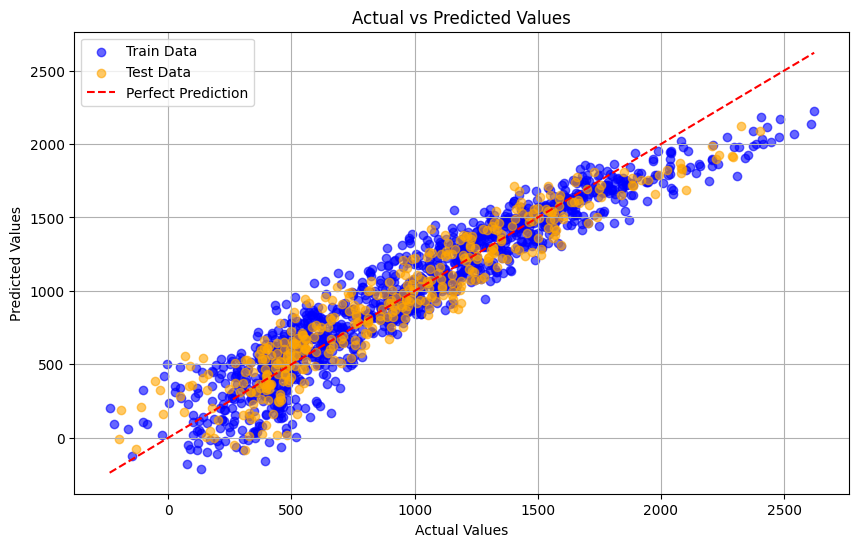
\includegraphics[width=0.9\textwidth]{data/regular.png} % Replace with your image file
    \caption{Dane oryginalne, MSE: $13607.09$}
    \end{minipage}
    \hspace{0.02\textwidth}
    \begin{minipage}[b]{0.48\textwidth}
        \centering
    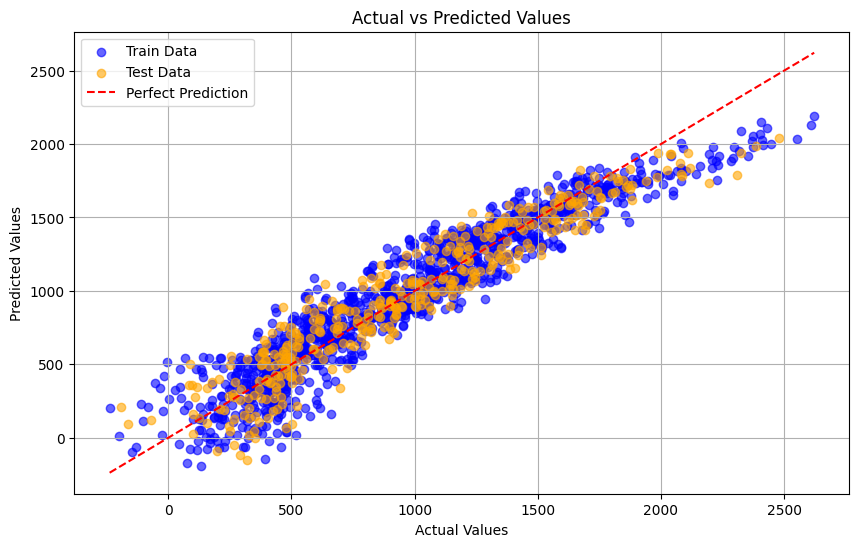
\includegraphics[width=0.9\textwidth]{data/standard.png} % Replace with your image file
    \caption{Dane ustandaryzowane, MSE: $13675.66$}
    \end{minipage}
\end{figure} \\
Standaryzacja jednak w klasycznym modelu regresji liniowej nie ma aż tak dużego znaczenia - ta której użyłem jest przekształceniem liniowym danych wejściowych, zatem nasz model może się nauczyć innych parametrów co doprowadzi go do podobnych rezultatów. Powyżej przedstawiam porównwanie wyników rozwiązania analitycznego na zbiorze testowym danych oryginalnych i ustandaryzowanych. \bigskip \\
Standaryzacja danych użyteczna jest jednak w momencie, gdy będziemy chcieli szerzej je analizować. Gdy ustandaryzujemy nasze dane, możemy na podstawie rozwiązania problemu regresji liniowej wnioskować (po rozmiarze parametrów) od jakich cech nasz wynik zależy najbardziej. Dodatkowo na ustandaryzowane dane możemy swobodnie aplikować funkcje bazowe i regularyzacje, jednocześnie nie przejmując się tym że skala konkretnych cech przyćmi pozostałe.



\section*{Algorytmy}
Podczas tego projektu zaimplementowałem dwie wersje algorytmu spadku wzdłuż gradientu. Pierwsza używała
pełnego zestawu danych treningowych - jedna iteracja to jedna epoka. W drugiej użyłem metody gradientu mini-batch. Przy \textbf{poprawnie} ustandaryzowanych danych odpowiednim \texttt{learning rate} okazał się być $\eta = 0.01$ $-$ po prostu gradient przy doborach różnych funkcji bazowych zbiegał odpowiednio szybko, ale nie był na tyle duży żeby algorytm przeskakiwał minimum czy wystrzeliwał do nieskończoności. Algorytm (de facto jeden, w dwóch trybach) miał różne warunki stopu $-$ można ustalić czy uzna model wytrenowany po $k$ iteracjach, czy w momencie gdy norma gradientu spadnie poniżej ustalonej liczby $\mu$. \bigskip \\
Na zajęciach wyprowadziliśmy fakt, że jeśli $\theta$ minimalizuję funkcję błędu z normalizacją grzbietową o parametrze $\lambda$, to $\theta = (X^TX + \lambda I)^{-1} X^Ty$, przy czym odwrotność tej macierzy zawsze istnieje dla $\lambda > 0$. Dlatego napisałem również algorytm wyznaczający rozwiązanie analityczne, przy czym macierz $X^TX$ nie zawsze jest odwracalna więc żeby wyznaczyć rozwiązanie bez normalizacji biorę $\lambda \rightarrow 0$. Poniżej zamieszczam wyniki otrzymane na zbiorze testowym za pomocą rozwiązania analitycznego dla różnych $\lambda$ (biorąc jako zbiór treningowy $ 60\%$ danych wejściowych) \\
\begin{table}[h!]
\centering
\begin{tabular}{|c|c|c|}
\hline
\(\lambda\) & Train Set MSE & Test Set MSE \\
\hline
\(1 \times 10^{-6}\) & 14358.6917 & 14980.0649 \\
0.1                 & 14358.6957 & 14980.8088 \\
0.2                 & 14358.7079 & 14981.5606 \\
0.5                 & 14358.7931 & 14983.8635 \\
1                   & 14359.0972 & 14987.8599 \\
2                   & 14360.3111 & 14996.4448 \\
5                   & 14368.7628 & 15026.8995 \\
10                  & 14398.6450 & 15093.0902 \\
20                  & 14515.9055 & 15281.6319 \\
50                  & 15294.8474 & 16264.2287 \\
100                 & 17821.7851 & 19099.6548 \\
1000                & 135659.7145 & 139351.7539 \\
100000              & 590708.4282 & 595069.9019 \\
\hline
\end{tabular}
\caption{MSE rozwiązania analitycznego dla różnych wartości \(\lambda\)}
\end{table} \biskip \\
W dalszej części tej sekcji chciałbym porównać skuteczność algorytmu \textbf{mini-batch} w porównaniu do klasycznego algorytmu regresji liniowej. Na początku sprawdźmy, jak sprawuje się klasyczny algorytm. Poniższe wykresy przedstawiają zmianę gradientu oraz MSE w kolejnych iteracjach. W tym wywołaniu dostałem MSE na zbiorze treningowym: $14124.78$, na testowym: $14630.03$, a gradient zbiegł do $0.04$.
\begin{figure}
    \centering
    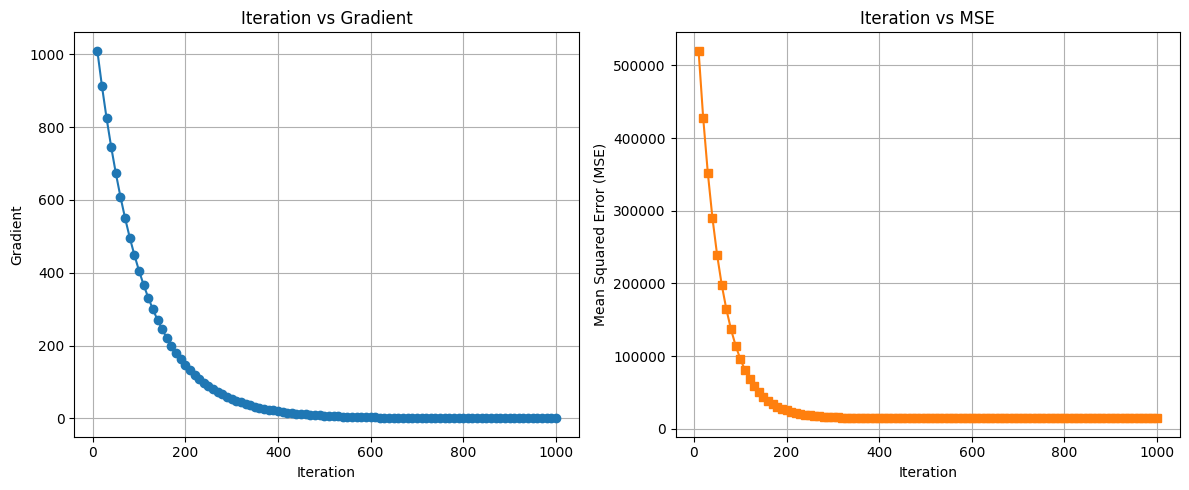
\includegraphics[width=0.9\textwidth]{data/itgradnormal.png}
    \caption{Gradient i MSE dla kolejnych iteracji, bez \textbf{mini-batch}}
\end{figure} \\
Jeśli chodzi o algorytm \textbf{mini-batch}, to ma on pewne ciekawe cechy które odkryłem podczas jego używania. Przez to że wybieramy dane w losowy sposób, to próbka którą dostajemy \texttt{względnie dobrze} symuluje średnią po wszystkich danych testowych. Jednak jest on ekstremalnie szybszy (miałem sytuacje gdy mini-batch trenował model podobnie efektywnie co zwykły gradient descent, ale robił to w $10$ sekund zamiast w $2$ minuty). Poniżej porównanie kilku przebiegów algorytmu \textbf{mini-batch} dla różnych ustawień rozmiaru pakietu.
\begin{figure}
    \centering
    \begin{minipage}[b]{0.48\textwidth}
    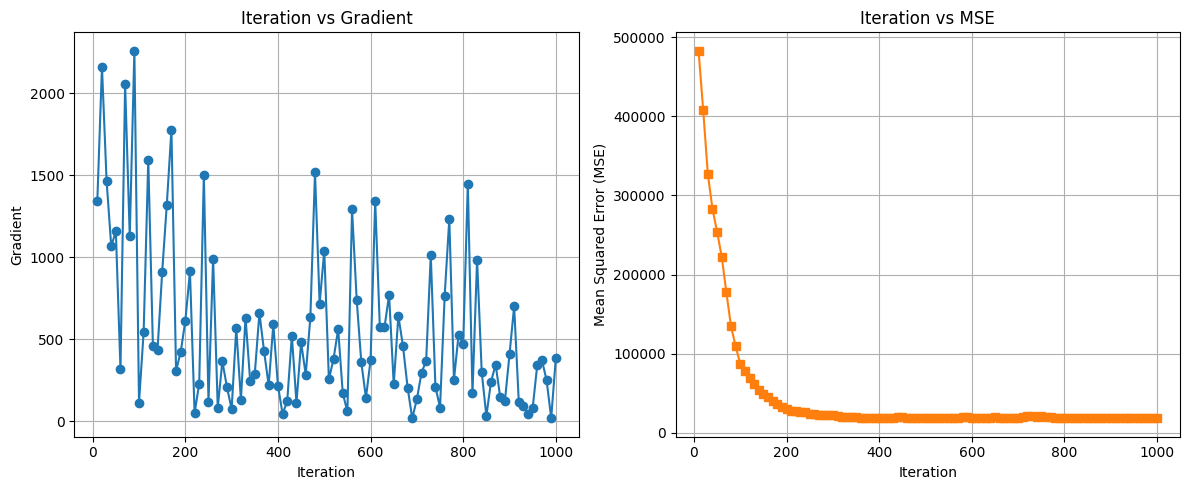
\includegraphics[width=0.9\textwidth]{data/b1.png}
    \caption{\texttt{batch size}$=1$, \texttt{MSE}$=14957.47$}
    \end{minipage}
     \hspace{0.02\textwidth}
    \begin{minipage}[b]{0.48\textwidth}
    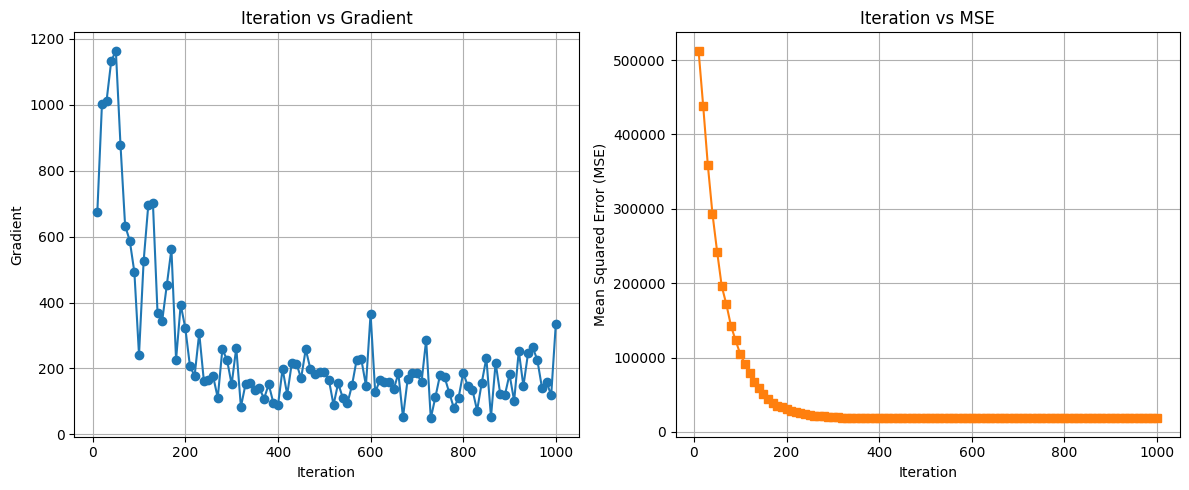
\includegraphics[width=0.9\textwidth]{data/b8.png}
    \caption{\texttt{batch size}$=8$, \texttt{MSE}$=14740.81$}
    \end{minipage}
    \hspace{0.02\textwidth}
    \begin{minipage}[b]{0.48\textwidth}
    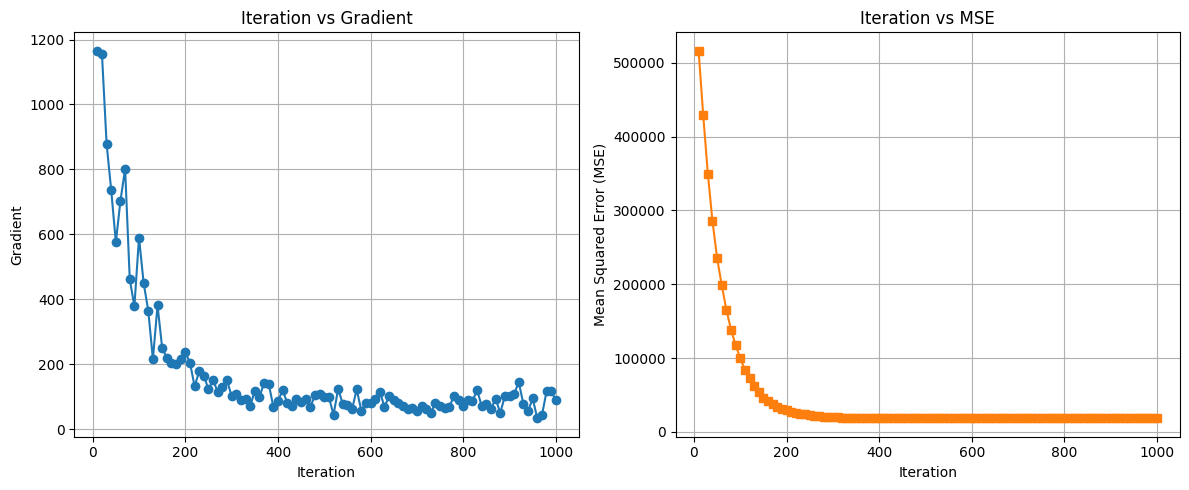
\includegraphics[width=0.9\textwidth]{data/b32.png}
    \caption{\texttt{batch size}$=32$, \texttt{MSE}$=14584.44$}
    \end{minipage}
     \hspace{0.02\textwidth}
    \begin{minipage}[b]{0.48\textwidth}
    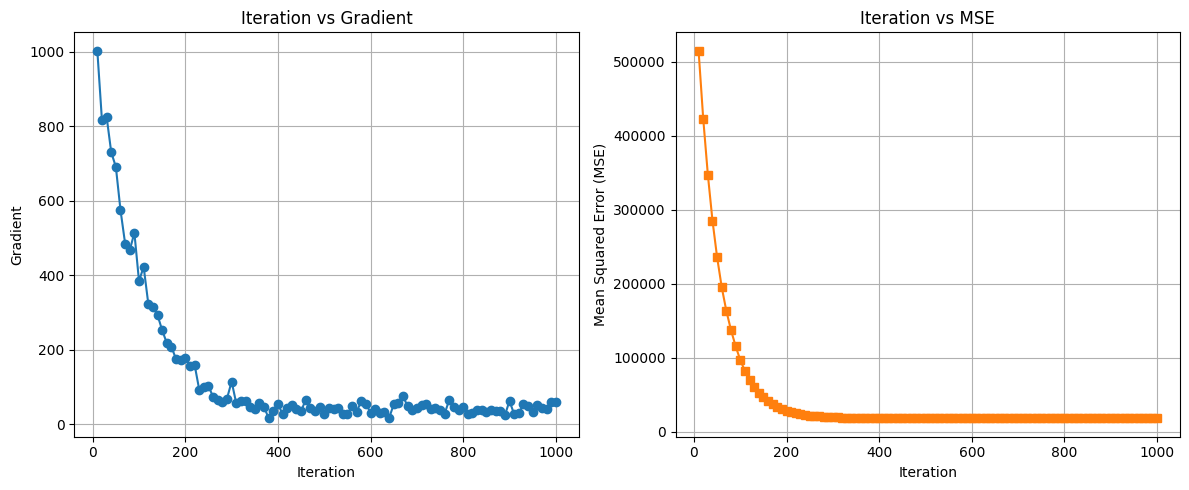
\includegraphics[width=0.9\textwidth]{data/b128.png}
    \caption{\texttt{batch size}$=128$, \texttt{MSE}$=14609.96$}
    \end{minipage}
\end{figure} \bigskip \\
Przez to, że w każdym przebiegu iteracji losujemy podzbiór danych na których się uczymy, to gradient w odróżnieniu do wersji bez \textbf{mini-batch} nie zbiega do 0, tylko drga zależnie od wylosowanego podzbioru. Nie przeszkadza to jednak w tym, aby nasz model poprawnie dopasowywał dane. Żeby zrównoważyć efektywność \textbf{mini-batch}, wybrałem \texttt{batch-size}$= 32$ do dalszych testów.

\FloatBarrier

\section*{Regularyzacja i wyznaczanie hiperparametrów}
Podczas trenowania modelu uwzględniłem również regularyzacje L1 i L2 oraz regularyzację z siecią elastyczną. Ąby wyznaczyć parametry regularyzacji, używam metody gradientu w wersji bez \textbf{mini-batch}, gdyż różnice dla różnych parametrów są często marginalne. Po rozdzieleniu danych na zbiór treningowy, walidacyjny i testowy porównuję wyniki na zbiorze walidacyjnym dla różnych parametrów $\lambda_1, \lambda_2 \in \{0, 0.0001, 0.001, 0.002, 0.005, 0.01, 0.02, 0.05, 0.1, 1, 2, 5, 10\}$. \bigskip \\
Okazuje się że gdy nie rozważamy funkcji bazowych to regularyzacja nie daje prawie żadnej poprawy gdy chodzi o przewidywanie naszych danych, gdyż nawet na danych treningowych ma problemy z dopasowaniem odpowiedniej płaszczyzny i nie zachodzi przeuczenie. Gdy będziemy jednak trenować nasz model dla wybranych funkcji bazowych, będziemy z niej korzystać żeby algorytm mógł dopasowywać się do danych bez overfittingu. Na wykresach poniżej widzimy, że model póki co osiąga najlepsze wyniki, gdy w ogóle nie korzystamy z regularyzacji.
\begin{figure}
    \centering
    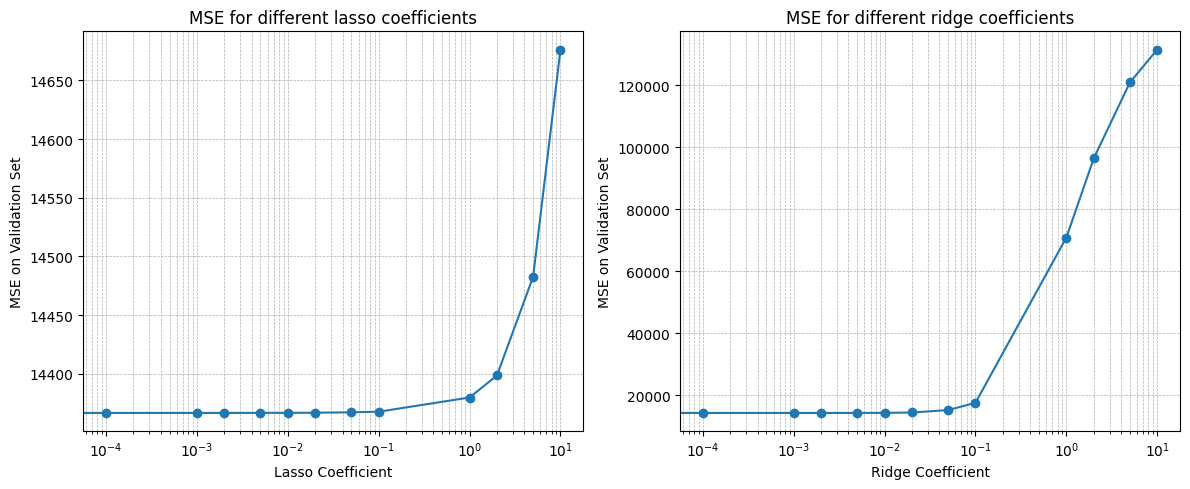
\includegraphics[width=0.9\textwidth]{data/valid_reg_coef.png}
    \caption{Wyniki dla różnych parametrów regularyzacji na zbiorze walidacyjnym}
\end{figure} \\
\FloatBarrier
\section*{Uczenie na frakcjach zbioru treningowego}
W tym rozdziale chciałbym przeanalizować, jak model poradzi sobie na różnych frakcjach zbioru treningowego. Analogicznie jak we wcześniejszej części dokumentu, będę stosował podział danych na zbiory w proporcji $0.6 : 0.2 : 0.2$. Dane które zebrałem zostały przygotowane w następujacy sposób: Mój algorytm miał $5$ przebiegów w których za każdym razem najpierw podzieliłem dane na zbiory, a potem odpaliłem algorytm regresji liniowej na różnych frakcjach zbioru treningowego i zebrałem wyniki. Na koniec uśredniłem wyniki dla każdej frakcji.

\begin{figure}[h!]
    \centering
    \begin{minipage}[b]{0.48\textwidth}
    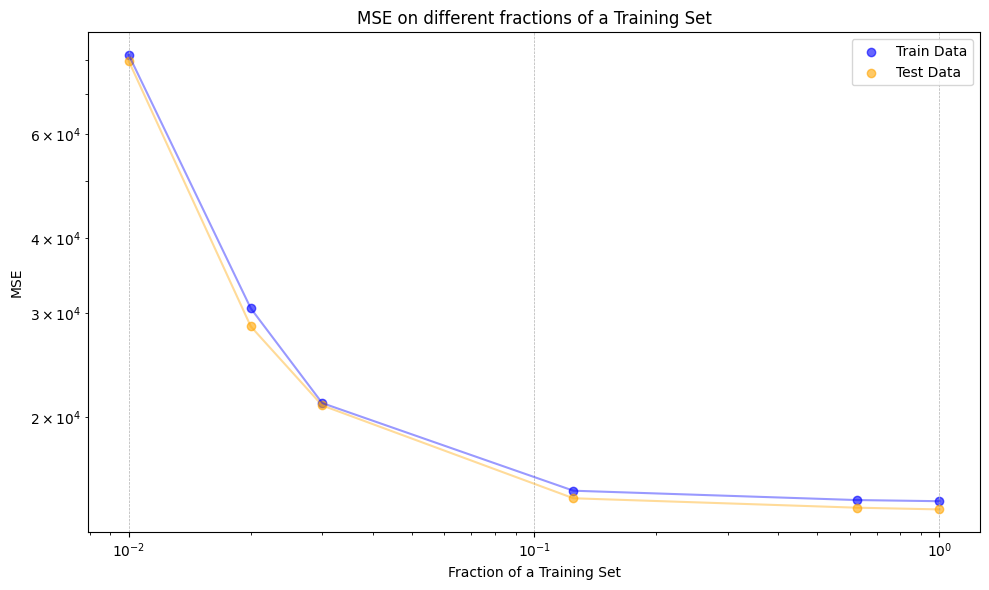
\includegraphics[width=0.9\textwidth]{data/fracgraph.png}
    \caption{Wyniki dla różnych frakcji zbioru treningowego}
    \end{minipage}
     \hspace{0.02\textwidth}
    \begin{minipage}[b]{0.48\textwidth}
    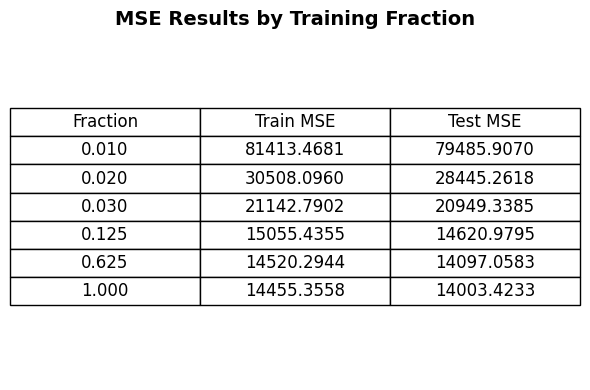
\includegraphics[width=0.9\textwidth]{data/fractable.png}
    \end{minipage}
\end{figure}
\FloatBarrier

Widzimy, że mimo początkowo ogromnej różnicy model radzi sobie nienajgorzej już, gdy korzystamy z $12.5 \% $ czy $62.5 \%$ zbioru treningowego. Spróbujmy teraz zbić nasz wynik za pomocą wykorzystania funkcji bazowych.

\section*{Szersza analiza danych}
Pierwszą rzeczą, od której zacząłem, było stworzenie macierzy korelacji (Pearsone'a) między cechami $x$ oraz wynikiem y na podstawie danych. Macierz ta mówi nam o stopniu zależności między poszczególnymi cechami i wynikiem. Dodatnia korelacja będzie nam mówić o tym że gdy jedna wartość rośnie to druga też, a ujemna, że gdy jedna wartość rośnie, to druga maleje. Poniżej przedstawiam tą macierz w formie heatmapy.

\begin{figure}[h!]
    \centering
    \begin{minipage}[b]{0.48\textwidth}
    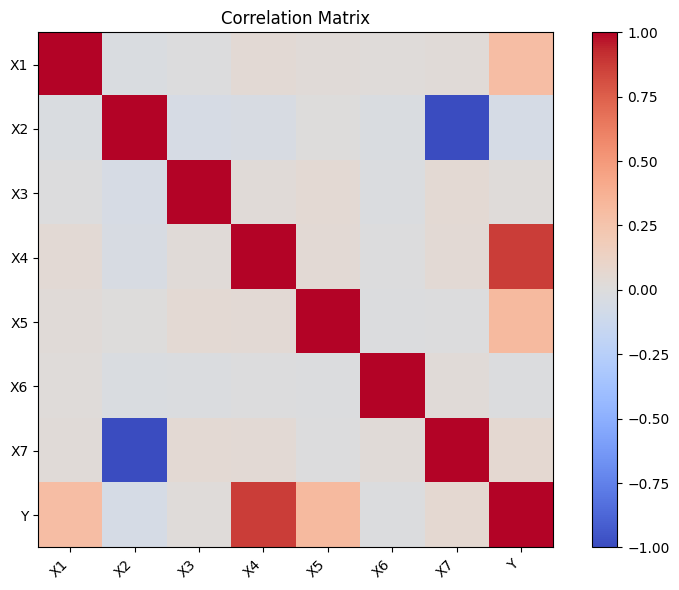
\includegraphics[width=0.9\textwidth]{data/corr.png}
    \caption{Macierz korelacji}
    \end{minipage} \hspace{}
    \begin{minipage}[b]{0.48\textwidth}
    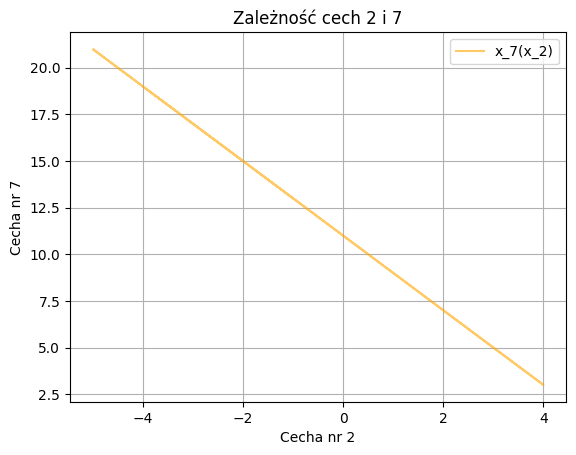
\includegraphics[width=0.9\textwidth]{data/linear27.png}
    \caption{Zależność $x_2$ i $x_7$}
    \end{minipage}
\end{figure} \\

Pierwsze, co bardzo się rzuca w oczy to to jak silnie skorelowane są cechy nr 2 i 7. Okazuje się, że w dostarczonych danych $x_7$ jest funkcją $x_2$, zatem jedna z tych cech jest nadmiarowa. Widzimy również, że wynik $y$ jest najbardziej skorelowany z cechami $x_1, x_4, x_5$, trochę słabiej z $x_7$ i $x_3$. Zatem moim strzałem będzie użycie funkcji bazowych $[x_1, x_3, x_4, x_5, x_6, x_7, x_1^2, x_4^2, x_5^2, x_1 \cdot x_4, x_1 \cdot x_5, x_4 \cdot x_5]$. Gradient zbiegał o wiele wolniej, więc puściłem algorytm na $5000$ iteracji. Otrzymałem \texttt{Train Set MSE = 8069.05} oraz \texttt{Test Set MSE = 8945.86}. Jednak używając funkcji bazowych $[W(x) : \deg(W) \leq 2]$ otrzymuję jeszcze lepsze MSE, \texttt{Train Set MSE = 4356.73, Test Set MSE = 4403.39}. Używając funkji bazowych $[W(x) : \deg(W) \leq 3]$ dostaję nieznaczną poprawę, \texttt{Train Set MSE: 3836.69, Test Set MSE: 4142.41}

\begin{figure}[h!]
    \centering
    \begin{minipage}[b]{0.48\textwidth}
    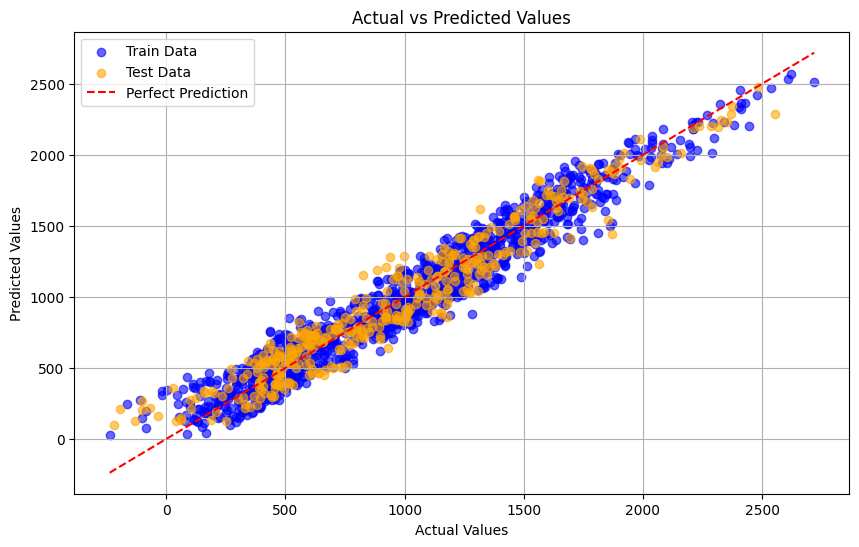
\includegraphics[width=0.9\textwidth]{data/first_custom.png}
    \caption{Wyniki pierwszej partii funkcji bazowych}
    \end{minipage} \hspace{}
    \begin{minipage}[b]{0.48\textwidth}
    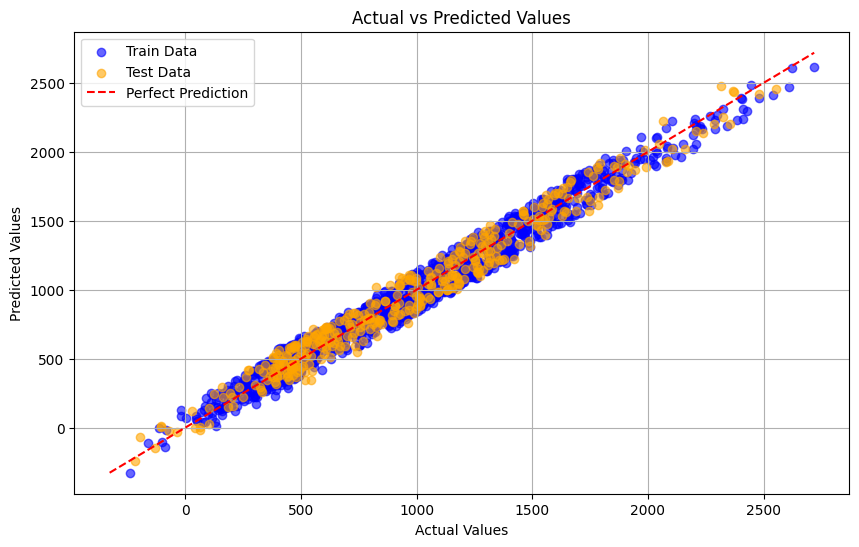
\includegraphics[width=0.9\textwidth]{data/third_custom.png}
    \caption{Wyniki trzeciej partii funkcji bazowych}
    \end{minipage}
\end{figure} \\

Cichym bohaterem okazał się tu być algorytm \textbf{mini-batch}, który znacząco poprawia szybkość działania algorytmu bez pogarszania jakości uczenia się. Widzimy zatem, że raczej nie chodzi o wielomiany trzeciego stopnia, więc spróbujmy dołożyć coś do tych drugiego.

\begin{figure}[h!]
    \centering

    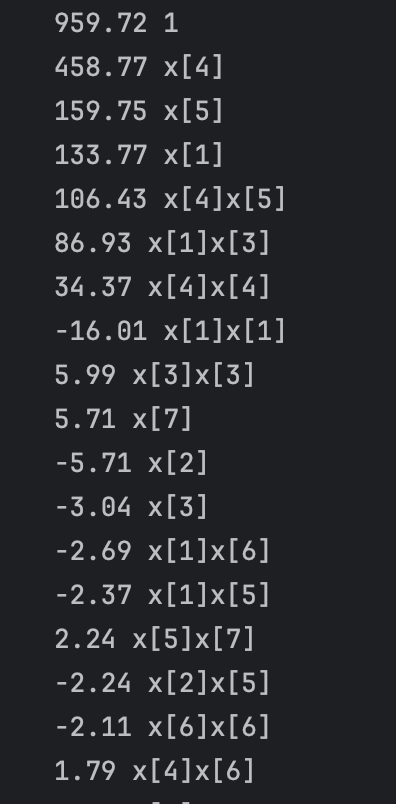
\includegraphics[width=0.25\textwidth]{data/sorted.png}
    \caption{Współczynniki $\theta$ przy kolejnych funkcjach bazowych}
\end{figure} \\

Wróćmy do przypadku z wielomianami 2 stopnia i przeanalizujmy parametry przy kolejnych funkcjach bazowych. Widzimy, że model szacuje że największą rolę grają kombinacje $x_1, x_2, x_4, x_5$ ale również $x_3^2$, którego nie uwzględniliśmy przy naszym pierwszym pomyśle. Wysokie współczynniki przy funkcjach liniowych dają mi pomysł, że warto spróbować do naszych cech dołożyć funkcje gaussowskie. \bigskip \\
Przetestowałem swoją hipotezę używając różnych funkcji bazowych postaci
\begin{center}
$[W(x) : \deg(W) \leq 2] \cup \bigcup_{i, \alpha}[g(x_i, \alpha)]$
\end{center}
Gdzie $g(x, \alpha) = \mathrm{e}^{-\frac{x^2}{\alpha^2}}$, dla każdej z nich w oparciu o zbiór walidacyjny wyznaczyłem parametry regularyzacji z siecią elastyczną. Trenowanie tego modelu wraz z wyznaczaniem hiperparametrów zaczęło schodzić wykładniczo długo (uznałem że użycie regularyzacji będzie przydatne, gdyż model zaczął overfitować się do zbioru treningowego). Jednak udało mi się w ten sposób znacząco zbić błąd i w końcu dotrenowałem model do wyników \texttt{Train Set MSE: 1291.55 Test Set MSE: 1294.79}. A oto funkcje bazowe których użyłem
\begin{center}
    $[W(x) : \deg(W) \leq 2] \cup \bigcup_{i\neq 2}[g(x_i, 0.01)]\cup \bigcup_{i\neq 2}[g(x_i, 0.5)]$
\end{center}


\begin{figure}[h!]
    \centering
    \begin{minipage}[b]{0.48\textwidth}
    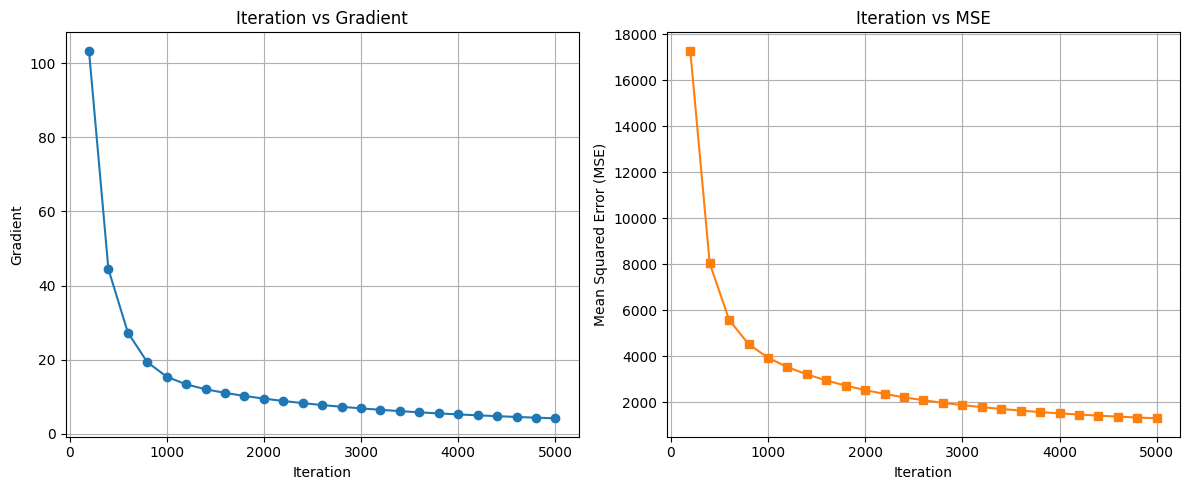
\includegraphics[width=0.9\textwidth]{data/finlc.png}
    \caption{Krzywa uczenia ostatecznego modelu}
    \end{minipage} \hspace{}
    \begin{minipage}[b]{0.48\textwidth}
    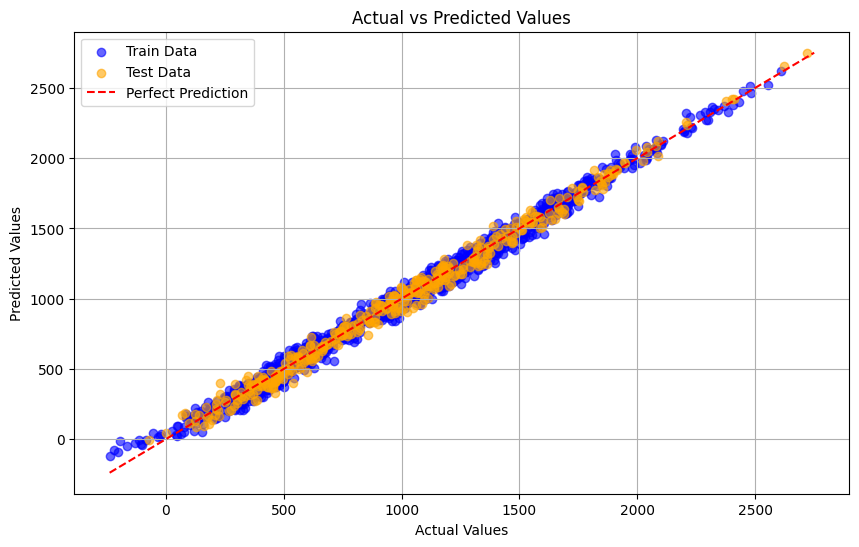
\includegraphics[width=0.9\textwidth]{data/finadjust.png}
    \caption{Wynik ostateczny}
    \end{minipage}
\end{figure} \\


\section*{Podsumowanie}
Podczas pracy z załączonymi danymi udało mi się zbliżyć do błędu $\approx 1294.79$. Po turbulencjach związanych z umiejętnościami kodowania udało mi się również przetestować moje rozwiązanie na konkursie.
\begin{figure}[h!]
    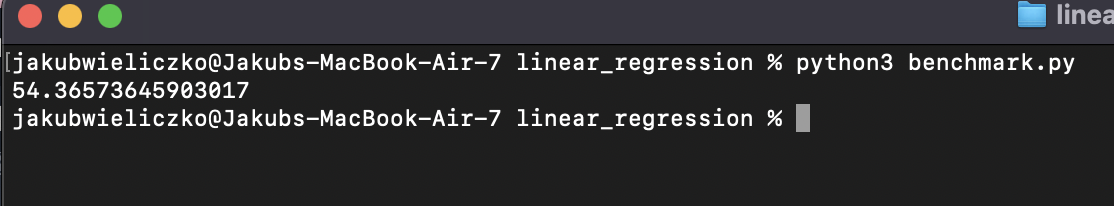
\includegraphics[width=0.9\textwidth]{data/benchmark.png}
    \caption{Benchmark jaki uzyskałem}
\end{figure} \\

\end{document}
